%%% 1206.tex

%% Copyright (C) 2012 LRDE.

%% Permission is granted to copy, distribute and/or modify this document
%% under the terms of the GNU Free Documentation License, Version 1.2
%% or any later version published by the Free Software Foundation;
%% with the Invariant Sections being just ``Copying this document'',
%% no Front-Cover Texts, and no Back-Cover Texts.

%% A copy of the license is provided in the file COPYING.DOC.

\documentclass{techrep} % You can pass the french option if you like.
\usepackage[T1]{fontenc}
\usepackage{amsmath, bm}
\usepackage{fancyhdr}
\usepackage{array}
\usepackage{stmaryrd}
\usepackage{graphicx}
\usepackage{gensymb}
\usepackage{vaucanson-g}
\usepackage{amsfonts}
\usepackage{float}
\usepackage{verbatim}
\usepackage{makeidx}
\usepackage{lmodern}
\usepackage{amsmath}
\usepackage{amsthm}
\usepackage{amsfonts}
\usepackage{tikz}
\usepackage{listings}

\usetikzlibrary{automata,positioning}
\title{SpeakerID - Spherical Discriminant Analysis}
\author{Victor Lenoir} \revision$LastChangedRevision: 2340 $
\date{January 2013} \email{lenoir@lrde.epita.fr}
%% \www{URL}{TEXT}

\definecolor{dkgreen}{rgb}{0,0.6,0}
\definecolor{gray}{rgb}{0.5,0.5,0.5}
\definecolor{mauve}{rgb}{0.58,0,0.82}

\lstset{ %
  language=Python,                % the language of the code
  basicstyle=\footnotesize,           % the size of the fonts that are used for the code
  numbers=left,                   % where to put the line-numbers
  numberstyle=\tiny\color{gray},  % the style that is used for the line-numbers
  stepnumber=2,                   % the step between two line-numbers. If it's 1, each line
  % will be numbered
  numbersep=5pt,                  % how far the line-numbers are from the code
  backgroundcolor=\color{white},      % choose the background color. You must add \usepackage{color}
  showspaces=false,               % show spaces adding particular underscores
  showstringspaces=false,         % underline spaces within strings
  showtabs=false,                 % show tabs within strings adding particular underscores
  frame=single,                   % adds a frame around the code
  rulecolor=\color{black},        % if not set, the frame-color may be changed on line-breaks within not-black text (e.g. commens (green here))
  tabsize=2,                      % sets default tabsize to 2 spaces
  captionpos=b,                   % sets the caption-position to bottom
  breaklines=true,                % sets automatic line breaking
  breakatwhitespace=false,        % sets if automatic breaks should only happen at whitespace
  title=\lstname,                   % show the filename of files included with \lstinputlisting;
  % also try caption instead of title
  keywordstyle=\color{blue},          % keyword style
  commentstyle=\color{dkgreen},       % comment style
  stringstyle=\color{mauve},         % string literal style
  escapeinside={\%*}{*)},            % if you want to add a comment within your code
  morekeywords={*,...}               % if you want to add more keywords to the set
}
%10 lines


\summary{ The purpose of a speaker verification system is to check
  whether an hypothesized speaker is really the author of a speech
  utterance. Currently, the best performances are performed using a
  mapping of each speaker utterance to a low dimensional vector called
  I-vector. The speaker verification score is computed thanks to a
  cosine distance between these two vectors representing both a
  speaker.


  In this paper, we describe a dimensionality reduction technique
  called Spherical Discriminant Analysis (SDA).  The goals of this
  projection are to maximize the cosine distance between different
  speaker's uterrances and minimize the cosine distance between same
  speaker's utterances; it has been shown that SDA subspace, which is
  more suitable for the cosine distance than Linear Discriminant
  Analysis (LDA), yields superior performance in face recognition
  task. We will compare the SDA subspace performance with the standard
  LDA approach.}

\frenchsummary{La r\^ole de la v\'erification de locuteur est de
  v\'erifier l'identit\'e pr\'esum\'ee d'un segment de parole. Actuellement,
  les meilleures performances sont obtenus par un mapping de chaque
  segment de parole d'un locuteur vers un vecteur appel\'e I-vector. Le
  score de la v\'erification de locuteur est calcul\'e par une distance
  cosine entre ces deux vecteurs repr\'esentant chacun un locuteur.

  Ce rapport d\'ecrit une technique de r\'eduction de dimension
  appel\'ee Spherical Discriminant Analysis (SDA). Les objectifs de
  cette projection sont de maximiser la distance cosinus entre deux
  locuteurs diff\'erents et de minimiser la distance cosinus entre
  deux m\^eme locuteurs; il a \'et\'e montr\'e que le sous-espace de
  la SDA, qui est plus appropri\'e pour la distance cosinus que la
  Linear Discriminant Analysis (LDA), obtient de meilleur performance
  en reconnaissance faciale. Nous allons comparer les performances
  obtenues par la SDA avec celles obtenues par la LDA.}

\keywords{speaker verification, dimensionality reduction, subspaces,
  ivector, cosine distance}

\begin{document}

\section*{Copying this document}
Copyright \copyright{} 2012 LRDE.

Permission is granted to copy, distribute and/or modify this document
under the terms of the GNU Free Documentation License, Version 1.2 or
any later version published by the Free Software Foundation; with the
Invariant Sections being just ``Copying this document'', no
Front-Cover Texts, and no Back-Cover Texts.

A copy of the license is provided in the file COPYING.DOC.

\tableofcontents

\newpage
%TODO: remerciements
\chapter*{Introduction}
%Une introduction avec le contexte général de votre travail, une
%description des problèmes auxquels vous voulez répondre et comment
%vous y répondez.  L’introduction doit capturer le lecteur et lui
%donner envie de lire la suite. Elle doit donner assez d’informations
%pour que celui-ci puisse comprendre l’intérêt de votre travail et la
%portée de vos résultats.  Plan
\chapter{Context: Speaker verification system}
%Présenter plus en détail le cadre de travail, la problématique, et
%l’existant.

%S’il y a des prérequis, des notions que devraient
%connaître le lecteur, c'est ici.

%Par exemple le projet Vaucanson a souvent besoin de revenir sur les
%bases des transducteurs; il est alors stupide de taper à nouveau
%cette introduction. Il vaut mieux maintenir une base commune, et
%clairement faire apparaître ses auteurs.


Nowadays, in a lot of secure applications, people have to prove their
own identity to go into a critical system. Most of these applications
are based on password authentications as in bank cash points or in the
access of some protected buildings. However, in such systems, a robber
can easily find the password and use it to gain access to the critical
area. For this reason, more and more authentication systems are based
on biometrical features like fingerprints, iris or voice which present
more inviolable features. Indeed, the study of these biometrical
features is an expanding research field. Furthermore, it is known that
fingerprints have been used extensively in criminal investigations for
a long time. Today, voice recognition systems are beginning to have a
legal status in some countries as a proof to authenticate a speaker on
a tape recording.  In this report, we consider the problem of voice
authentication, generally called the speaker verification
problem. More precisely, we focus on the text-independent speaker
verification i.e we do not consider the uttered text.\\\\ In our
speaker verification task, speakers are first modeled from enrollment
data coming from phone recordings. During the verification task, these
models enable to check whether a segment of speech is uttered by an
hypothesized speaker. For a few years, the community has been more and
more interested in resolving this verification problem even if the
enrollment conditions are different during the training step and the
testing step.

\section{Speaker verification system}

\tikzstyle{cont}=[shape=rectangle,minimum
  size=1.0cm,draw=blue!70,fill=blue!30,font=\small]

\tikzstyle{contred}=[shape=rectangle,minimum
  size=1.0cm,draw=red!70,fill=red!30,font=\small]

\begin{center}
  \begin{tikzpicture}[scale=0.8,font=\scriptsize]
    \node[cont,initial above] (s1) at (0,0) {Audio signal};
    \node[cont] (s2) at (0,-2) {Audio features}
    edge [<-] node[left] {Features extraction} (s1);
    \node[cont] (s3) at (0,-4) {Speaker features}
    edge [<-] node[left] {Voice Activity Detection/Speaker diarization} (s2);
    \node[cont] (s4) at (0,-6) {Speaker model}
    edge [<-] node[left] {Modeling} (s3);
    \node[cont] (s5) at (0,-8) {Low-dimensional speaker model}
    edge [<-] node[auto] {\textcolor{red}{Dimension reduction}} (s4);
    \node[cont] (s6) at (5,-10) {Low-dimensional speaker model};
    \node[cont] (s7) at (0,-10) {Score}
    edge [<-] node[auto] {Scoring} (s5)
    edge [<-] node[auto] {Scoring} (s6);
    \node[cont] (s8) at (0,-12) {Decision}
    edge [<-] node[auto] {Threshold} (s7);
  \end{tikzpicture}
\end{center}

In our system:
\begin{description}
\item[Features] Cepstral vectors (acoustic parameters);
\item[Speaker model] Identity-Vector (Ivector, 600-dim vector which
  represents the speaker);
\item[Low-dimensional speaker model] 400-dim vector obtained by
  Probabilistic Linear Discriminant Analysis (PLDA)
\item[Score] Cosine-Distance between two low-dimensional speaker models;
\item[Decision] Whether the speakers are the same or not.
\end{description}

\section{Dimension reduction}

In this paper, we only have interest in the dimension reduction
process. The idea is to find a subspace which yields superior
classification performance than the original space. One of the most
known dimension reduction technique is the Linear Discriminant
Analysis (LDA).

The goals of the LDA is to maximize the between class (different
speakers) covariance while minimizing the within class (same speakers)
covariance. Therefore, in the subspace, two different speakers will
have a greater euclidean distance than in the original space.

A common approach to project vectors into a better subspace is to
train a projection matrix offline using a training database with a lot
of classes (different speakers). Then, during the speaker verification process, we only
have to project our vectors using our newly learned projection matrix.

\chapter{Spherical Discriminant Analysis}



In this chapter, we will present a dimension reduction technique
called Spherical Discriminant Analysis (SDA). This technique is quite
similar to the LDA but is using the cosine distance instead of the
euclidean distance.

\newcommand{\argmax}[1]{\smash{\mathop{{\rm argmax}}\limits_{W}}\, #1}
\newcommand{\argmin}[1]{\smash{\mathop{{\rm argmin}}\limits_{W}}\, #1}

\section{Cosine distance}

The cosine distance is a well-used distance which only considers the
direction of a data point and not its norm like the usual euclidian distance.

$$a.b = ||a||.||b||. \cos{\theta}$$
$$\text{cosine similarity} = \cos{\theta} = \frac{a.b}{||a||.||b||}$$
$$\text{cosine distance} = 1 - \cos{\theta} = 1 - \frac{a.b}{||a||.||b||}$$

\begin{figure}[H]
  \centering
  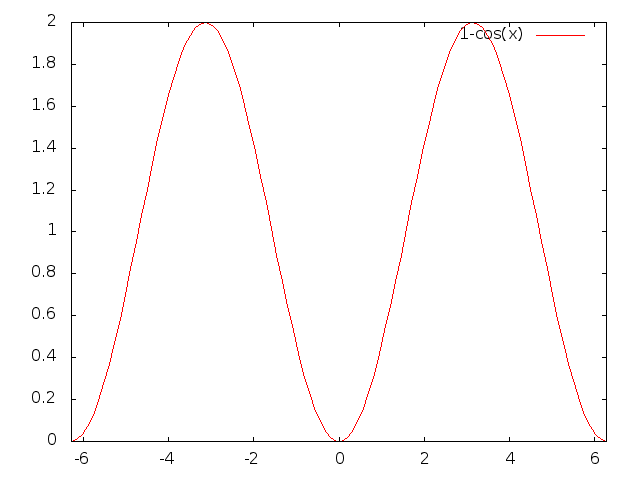
\includegraphics[width=250px]{cosine_distance}
  \caption{Cosine distance plot where $x$ is the angle between two
    vectors.}
  \label{cosine_distance}
\end{figure}

\section{Gradient descent}

The gradient descent is one of the most used optimization method. It's
an iterative method which consists in using the derivative at each
iteration to head towards the local optimum (minimum or maximum).

\begin{figure}[H]
  \centering
  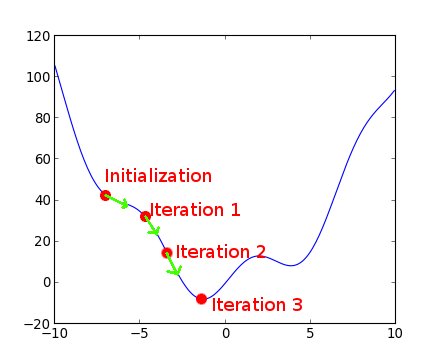
\includegraphics[width=250px]{gradient_descent}
  \caption{Gradient descent with only one parameter. The local minimum found is -10 with parameter -1.}
  \label{gradient_descent}
\end{figure}

\begin{figure}[H]
  \begin{lstlisting}[frame=single]
    while not converge:
        for parameter in parameters:
                parameter = parameter - alpha * derivative_parameter(parameters);
  \end{lstlisting}
  \caption{Gradient-descent algorithm}
  \label{algo_gradient_descent}
\end{figure}

In the algorithm \ref{algo_gradient_descent}, the alpha refers to the
step. If the step is too low, the convergence will be very
slow. However, if the step is too high, the algorithm may not
converged. The big issue in the gradient descent method is to find the
step suitable for the problem.

Fortunately, there are other gradient descent methods which don't
require to choose a step.

\subsection{Resilient backpropagation}

The idea behing the resilient backpropagation (Rprop) is to have
dynamic steps unique to each parameters.
The update rules of these steps are:
\begin{itemize}
\item Speed up: Increase the step when the previous derivative and the
  current derivative have the same sign;
\item Slow down: Decrease the step otherwise.
\end{itemize}

This method has two advantages:
\begin{itemize}
\item We don't have to choose a step;
\item The convergence may be faster thanks to the speed ups.
\end{itemize}
\section{Principle}

We have previously seen that we are using a cosine distance between
two low-dimensional vectors to compute a score between two speaker's
utterances. The idea behind the Spherical Discriminant Analysis is
similar to the idea of the Linear Discriminant Analysis: we want to
maximize the distance between two different speakers while minimizing
the distance between two same speakers. The only difference is that we
are using the cosine distance instead of the euclidean distance so
that the scoring, hence the decision, is more accurate.\\ Concretely,
we want to find a projection matrix $W$ from the I-vector space to our
SDA subspace such as:

$$W = \argmin(S_b - S_w)$$
with
$$S_b =
\frac{1}{c(c-1)}\sum_{m=1}^c\sum_{n=1}^c\frac{1}{|D_m||D_n|}\sum_{\substack{x_i
    \in D_m \\ x_j \in D_n}}
\frac{x_i^TWW^Tx_j}{\sqrt{x_i^TWW^Tx_i}\sqrt{x_j^TWW^Tx_j}} (m \neq
n)$$ and
$$S_w = \frac{1}{c}\sum_{i=1}^c\frac{1}{|D_i|^2}\sum_{x_j,x_k \in D_i}
\frac{x_j^TWW^Tx_k}{\sqrt{x_j^TWW^Tx_j}\sqrt{x_k^TWW^Tx_k}}$$
where:
\begin{itemize}
  \item $c$: number of speakers;
  \item $D_i$: I-vectors of the speaker $i$;
  \item $|D_i|$: number of I-vectors of the speaker $i$.
\end{itemize}

$S_b$ is the between-class cosine similarity of the projected
space. It is simply the average cosine similarity (opposite of the
cosine distance) between the data points of different classes. In this
situation it is the average cosine similarity between the speech
utterances of different speakers.

Similarly, $S_w$ is the within-class cosine similarity of the
projected space. It is the average cosine similarity between the
speech utterances of same speakers.\\
By finding a projection matrix $W$ minimizing the between-class cosine
similarity while maximizing the within-class cosine similarity we find
a subspace suitable for cosine distance scoring.

\section{Algorithm}

In order to find this matrix, we have to find the derivative of $S_b -
S_w$ in order to apply a gradient descent method. % phrase bizarre

Let $F(W) = S_b - S_w$, then the derivative is defined as below:
$$\frac{\partial{F(W)}}{\partial{W}} =
2\sum_{i\neq{}j}\left[\frac{f_{ij}x_ix_i^TW}{f_i^3f_j} +
  \frac{f_{ij}x_jx_j^TW}{f_j^3f_i} - \frac{x_ix_j^TW + x_jx_i^TW}{f_if_j}\right]s_{ij}$$
Where:
\begin{itemize}
\item $f_{ij} = x_i^TWW^Tx_j$
\item $f_i = \sqrt{x_i^TWW^Tx_i}$
\item $s_{ij} = \frac{1}{c|D_i||D_i|}$ if $x_i$ and $x_j$ belong to the same class
\item $s_{ij} = -\frac{1}{c(c-1)|D_i||D_j|}$ otherwise
\end{itemize}

We now only have to find the projection matrix $W$ which minimize
$F(W)$ using the previously seen gradient descent method with the
derivative $\frac{\partial{F(W)}}{\partial{W}}$.
%\subsection{Demonstration of the derivative}


\subsection{Example}

Let us have a small experiment to understand and observe the
convergence of this algorithm.  For this experiment we only have three
different speakers and the subspace dimension is chosen to be two in
order to be able to plot the projected data.

Once the projection matrix $W$ is computed, the projection is done by:
$$y_i = \frac{W^Tx_i}{||W^Tx_i||}$$ The normalization term is not
mandatory for we use the cosine distance (which normalizes) but it
gives a better idea on the plot of the cosine distance.

\begin{figure}[H]
  \centering
  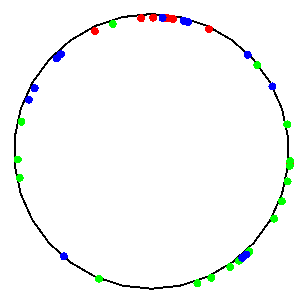
\includegraphics[width=150px]{draw0}
  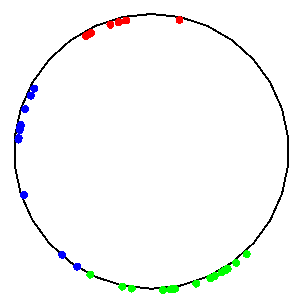
\includegraphics[width=150px]{draw1}
  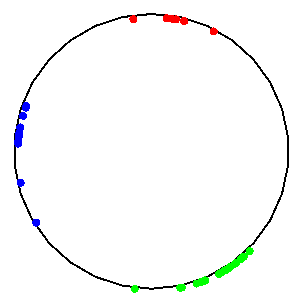
\includegraphics[width=150px]{draw2}
  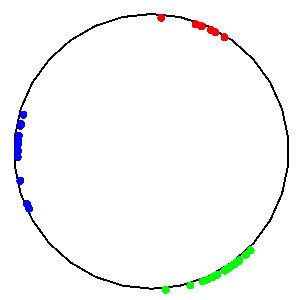
\includegraphics[width=150px]{draw3}
  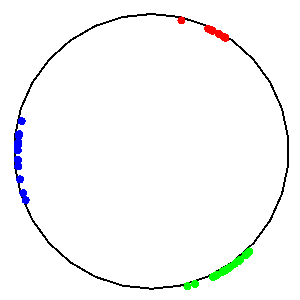
\includegraphics[width=150px]{draw4}
  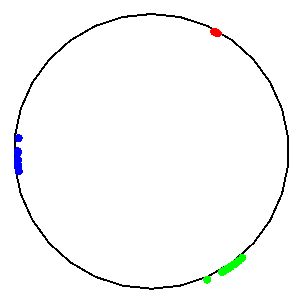
\includegraphics[width=150px]{draw8}
  \caption{Projected data plots by the randomly intialiazed matrix and
    by the matrix after 1, 2, 3, 4 and 8 iterations. A data point is a speech utterance and a speaker is
represented by a color.}
  \label{draws}
\end{figure}


The projected data is on a circle due to the data normalization.  We can
observe in the figure \ref{draws} that, over the iterations, the
average distance between the different speakers increased while the
average distance between the same speakers decreased.

\section{Implementation}
In this part, I will talk about the implementation specifications,
problems and solutions found.

\subsection{Specifications}

The implementation was made in C++ using the library blas for matrix
computations.

%talk about matrix class? YES.

\subsection{Problems}

%CPU
%RAM



\chapter{Experiments and results}
\section{Experiments}
\section{Results}
\section{Discuss}
% Previous work, Related work, future work
\chapter*{Conclusion}
%Quelques paragraphes. Une conclusion qui résume clairement le contenu
%de votre rédaction, dans le même ordre que le contenu présenté était
%détaillé. La conclusion doit ensuite mettre l’accent sur les
%principaux intérêts / fonctionnalités de ce que vous avez présenté et
%mettre en avant votre travail.  Ne pas se contenter de faire une
%resucée du résumé. D’ailleurs, ce n’est pas une «synthèse», c’est une
%«conclusion». En d’autres termes, ne pas s’arrêter à un résumé de
%l’article, mais finir en ouvrant le débat : quelles pistes restent
%encore à explorer, quels nouvelles questions ou problèmes se posent,
%quels autres sujets semblent liés etc.

\bibliography{final_report} \nocite{*}
\end{document}

%%% 1206.tex ends here.
